\documentclass[handout]{beamer}
% \documentclass{beamer}

%%
%%
%%
% From http://tex.stackexchange.com/questions/2072/beamer-navigation-circles-without-subsections
% Solution #2 or 3:
% \usepackage{etoolbox}
% \makeatletter
% % replace the subsection number test with a test that always returns true
% \patchcmd{\slideentry}{\ifnum#2>0}{\ifnum2>0}{}{\@error{unable to patch}}%
% \makeatother
% Solution #1:
\usepackage{remreset}% tiny package containing just the \@removefromreset command
\makeatletter
\@removefromreset{subsection}{section}
\makeatother
\setcounter{subsection}{1}


\usepackage{etex}
\usepackage{pgf}
\usepackage{tikz}
\usepackage{url}
\usepackage{amsmath}
\usepackage{color}
% \definecolor{red}{rgb}{1,0,0}
\usepackage{ulem}
% \usepackage{booktabs}
\usepackage{colortbl,booktabs}
\renewcommand*{\thefootnote}{\fnsymbol{footnote}}
\usepackage{fancybox}
\usepackage[framemethod=TikZ]{mdframed}
\mdfdefinestyle{FactStyle}{%
  outerlinewidth=0.5,
  roundcorner=1pt,
  leftmargin=1cm,
  linecolor=blue,
  outerlinecolor=blue!70!black,
  backgroundcolor=yellow!40
}
\usepackage{cancel}

  \newcommand\Warning{%
    \makebox[2.4em][c]{%
      \makebox[0pt][c]{\raisebox{.2em}{\Large!}}%
      \makebox[0pt][c]{\color{red}\Huge$\bigtriangleup$}}}%

\usepackage{stackengine}
\usepackage{scalerel}
\usepackage{xcolor}
  \newcommand\dangersign[1][2ex]{%
    \renewcommand\stacktype{L}%
    \scaleto{\stackon[1.3pt]{\color{red}$\triangle$}{\tiny !}}{#1}%
  }



\usepackage{dcolumn}
\newcolumntype{d}[1]{D{.}{.}{#1}}

% From
% http://tex.stackexchange.com/questions/109900/how-can-i-box-multiple-aligned-equations
\usepackage{empheq}
\usepackage{tcolorbox}  \newtcbox{\othermathbox}[1][]{%
  nobeforeafter, tcbox raise base, 
  colback=black!10, colframe=red!30, 
  left=1em, top=0.5em, right=1em, bottom=0.5em}

\newcommand\blue{\color{blue}}
\newcommand\red{\color{red}}
\newcommand\green{\color{green!75!black}}
\newcommand\purple{\color{purple}}
\newcommand\bluegreen{\color{blue!75!green}}
\newcommand\orange{\color{orange}}
\newcommand\redgreen{\color{red!50!green}}
\newcommand\grey{\color{black}}
\newcommand\gap{\vspace{.1in}}
\newcommand\nb{${\red\bullet}\ $}
\newcommand\halfgap{\vspace{.05in}}
\newcommand\divideline{\line(1,0){352}}
\usepackage{marvosym} % for \Smiley

\newcommand{\bluealert}[1]{{\blue\textbf{#1}}}

% \usepackage{beamerthemesplit} %Key package for beamer
\usetheme{Singapore}
% \usetheme{Szeged}
% \usetheme{Garfield}
% \usetheme{CambridgeUS}
% \usenavigationsymbolstemplate{} %Gets rid of slide navigation symbols


\setbeamercolor{separation line}{use=structure,bg=structure.fg!50!bg}
% \begin{beamercolorbox}[colsep=0.5pt]
%   {upper separation line foot}
% \end{beamercolorbox}



\makeatletter
\setbeamertemplate{footline}
{
  \leavevmode%
  \hbox{%
% \begin{beamercolorbox}[colsep=0.5pt]
%   {upper separation line foot}
% \end{beamercolorbox}


  \begin{beamercolorbox}[wd=.5\paperwidth,ht=2.25ex,dp=2ex,colsep=0.5pt]%
    {upper separation line foot}
    \usebeamerfont{author in head/foot}%
    \hspace*{2ex}\insertshortdate:\ \insertshorttitle
  \end{beamercolorbox}%
  \begin{beamercolorbox}[wd=.5\paperwidth,ht=2.25ex,dp=2ex,right]{title in head/foot}%
    \usebeamerfont{title in head/foot}
    {\insertshortauthor}\hspace*{2ex}
  \end{beamercolorbox}}%
  % \begin{beamercolorbox}[wd=.333333\paperwidth,ht=2.25ex,dp=2ex,right]{date in head/foot}%
  %   \usebeamerfont{date in head/foot}\insertshortdate{}\hspace*{2em}
  %   \insertframenumber{} / \inserttotalframenumber\hspace*{2ex} 
  % \end{beamercolorbox}%
  \vskip0pt%
}
\makeatother

\usetikzlibrary{decorations.markings}
\usetikzlibrary{arrows}


\title{Final Exam Review}
\author{Peter Garfield, UCSB Mathematics}
\date{March 15, 2017}
%\institute{}


\useinnertheme{default}

\usefonttheme{serif}
% \usecolortheme{rose}
% \usecolortheme{whale}
% \usecolortheme{orchid}
\usecolortheme{crane}
% \usecolortheme{dolphin}


%TEMPLATE
\setbeamertemplate{navigation symbols}{}

\setbeamertemplate{note page}[compress]

\setbeamertemplate{frametitle}{
  \vspace{0.5em}
  % \begin{centering}
  {\huge\blue\textbf{\textmd{\insertframetitle}}}
  \par
  % \end{centering}
}

% From http://tex.stackexchange.com/questions/7032/good-way-to-make-textcircled-numbers:
\newcommand*\circled[1]{\tikz[baseline=(char.base)]{\node[shape=circle,draw,fill=orange,inner sep=1pt] (char) {#1};}} 
% \renewcommand{\labelenumi}{\circled{\textbf{\arabic{enumi}}}}

\let\olddescription\description
\let\oldenddescription\enddescription
\usepackage{enumitem}
\let\description\olddescription
\let\enddescription\oldenddescription

% \usepackage[loadonly]{enumitem}
\setlist[enumerate,1]{label=\colorbox{orange}{\arabic*.},font=\bfseries}
%\setlist[enumerate,2]{label=\colorbox{blue!25}{(\alph*)},font=\bfseries}
% \setlist[enumerate,1]{label=\arabic*.,font=\bfseries}
\setlist[itemize,1]{label=\red$\bullet$}
\setlist[itemize,2]{label=\blue$\bullet$}

\newcommand\answer[1]{\fbox{#1}}
% \renewcommand\answer[1]{}

\newcommand{\antilog}{\operatorname{antilog}}







\title{}
\title{Optimization}
\date{June 5, 2017}


\begin{document}
\small

\section*{Administration}

\frame{
  \frametitle{Office Hours!}
  % \ \vspace*{0.25in}

  {\Large{}Instructor:}\\
  \ \hspace*{0.2in} Peter M.\ Garfield, \url{garfield@math.ucsb.edu}\\[0.25em]

  {\Large{}Office Hours:}\\
  \ \hspace*{0.2in} Mondays 2--3\textsc{pm}\\
  \ \hspace*{0.2in} Tuesdays 10:30--11:30\textsc{am}\\
  \ \hspace*{0.2in} Thursdays 1--2\textsc{pm}\\
  \ \hspace*{0.2in} or by appointment \\[0.25em]

  {\Large{}Office:}\\
  \ \hspace*{0.2in} South Hall 6510\\[0.5em]

  \copyright\ 2017\ Daryl Cooper, Peter M.\ Garfield

  % \vspace*{2in}
}

\section{Max / Min Review}
\frame{
  \frametitle{How To Find A Max / Min}

  \begin{mdframed}[style=FactStyle]
    \begin{itemize}
    \item[{\red(1)}] Find $f{\red '}(x)$

    \item[{\red(2)}] Solve $f{\red '}(x)=0.$ This is the $x$ value
      that gives the max / min. 

    \item[{\red(3)}] To find the maximum / minimum plug the value of $x$ found
      in {\red(2)}\ back into $f(x)$. 

    \end{itemize}
  \end{mdframed}
  \vspace*{0.5in}
  \pause

  \alert{Example:}\ Use this method to find the $x$-value where
  \emph{maximum}\ of the function $f(x)=5x-e^{2x}$ occurs.
  \begin{center}
    A $=0$
    \quad 
    B $= \ln(5)$
    \quad 
    C $= 2\ln(5)$
    \quad 
    D $= 2\ln(5/2)$
    \quad 
    E $= \ln(5/2)/2$
    \pause
  \end{center}
  \alert{Answer:}\ \answer{E}
  \vspace*{1in}


}

\section{Word Problems}

\frame{
  \frametitle{Word Problem \#1 (a re-run!)}

  A fenced garden with an area of $1000\ \text{m}^2$  will be made in
  the shape of a rectangle. It will be surrounded on all four sides by
  a fence. Three sides are wood fence, and the remaining side is a
  brick wall.
  \begin{itemize}
  \item The wood fence costs \$5 per meter length.
  \item The brick wall costs \$20 per meter length.
    \pause
  \item $C=$ total cost of the fence and brick wall
  \item $L=$ length of the brick wall
  \item $W=$ width of the other side 
  \end{itemize}
  \begin{enumerate}
  \item[\colorbox{blue!50}{(a)}] Find a formula for $C$ in terms of only $L$.
    \vspace*{-0.5em}

    \begin{center}
      A $= 2W + 2L$
      \quad 
      B $= 2000L^{-1}+2L$
      \quad 
      C $= 25L +10000L^{-1}$\\[0.5em] 
      % 
      \ \quad
      D $= 20L + 10000WL^{-1}$
      \quad 
      E $= 5L + 3000$
      \pause
      \quad
      \answer{C}
    \end{center}
    % \bigskip

  \item[\colorbox{blue!50}{(b)}]
    What length of brick wall gives lowest cost?
    \vspace*{-0.5em}

    \begin{center}
      A $= 20$
      \quad 
      B $= 40$
      \quad 
      C $= 50$
      \quad 
      D $= 100$
      \quad 
      E $= 25$
      \pause
      \quad
      \answer{A}
    \end{center}
  \end{enumerate}

}




\frame{ 
  \frametitle{Word Problem \#2} 

  A rectangular field is surrounded by fence. It is divided into 4
  equal
  \begin{center}
    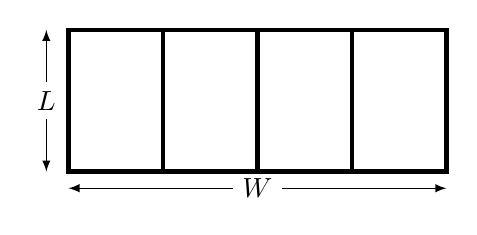
\begin{tikzpicture}[x=12mm,y=6mm,>=latex]
      \draw[thin,black,<->]  (-8pt,0) -- (-8pt,3) node[midway,fill=white] {$L$};
      \draw[thin,black,<->]  (0,-6pt) -- (4,-6pt) node[midway,fill=white] {$W$};
      \draw[ultra thick,black] (1,0) -- (1,3);
      \draw[ultra thick,black] (2,0) -- (2,3);
      \draw[ultra thick,black] (3,0) -- (3,3);
      \draw[ultra thick,black] (0,0) rectangle (4,3);
    \end{tikzpicture}
  \end{center}
  parts by 3 more dividing fences all parallel to one side of the
  field.
  \bigskip

  \begin{enumerate}
  \item[\colorbox{blue!50}{(a)}]\ 
    What is the total length of all the fence needed?
    \begin{center}
      A $= 2L+2W$
      \quad 
      B $= LW$
      \quad
      C $= 5LW$ \\[0.5em]
      \ 
      \quad \quad \quad 
      D $= L+W$
      \quad
      E $= 5L+2W$
      \pause
      \quad \quad \quad 
      \fbox{E}
    \end{center}
    \vspace*{-0.5em}

  \item[\colorbox{blue!50}{(b)}]\ 
    The field must have an area of $1000\ \text{m}^2$.
    Express $W$ in terms of $L$. 
    \begin{center}
      A\ $1000-L$
      \quad 
      B\ $1000L$
      \quad 
      C\ $1000/L$
      \quad 
      D\ $1000+L$
      \pause
      \quad
      \fbox{C}
    \end{center}
  \end{enumerate}
  % \vspace{2in}

}

\frame{ 
  \frametitle{Word Problem \#2 (cont'd)}

  A rectangular field is surrounded by fence. It is divided into 4
  equal
  \begin{center}
    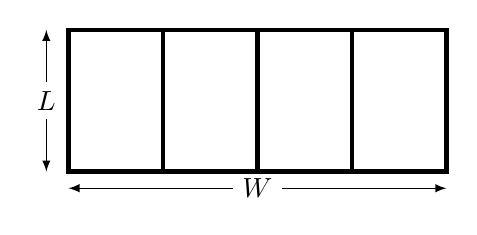
\begin{tikzpicture}[x=12mm,y=6mm,>=latex]
      \draw[thin,black,<->]  (-8pt,0) -- (-8pt,3) node[midway,fill=white] {$L$};
      \draw[thin,black,<->]  (0,-6pt) -- (4,-6pt) node[midway,fill=white] {$W$};
      \draw[ultra thick,black] (1,0) -- (1,3);
      \draw[ultra thick,black] (2,0) -- (2,3);
      \draw[ultra thick,black] (3,0) -- (3,3);
      \draw[ultra thick,black] (0,0) rectangle (4,3);
    \end{tikzpicture}
  \end{center}
  parts by 3 more dividing fences all parallel to one side of the
  field.
  \bigskip

  \begin{enumerate}
  \item[\colorbox{blue!50}{(c)}]\ 
    Express the total length of all the fence needed in terms of $L$.
    \begin{center}
      A $= 5L+1000$
      \quad 
      B $=  5L + 2000/L$
      \quad 
      C $= 5L+2/L$
      \quad
      \pause
      \fbox{B}
    \end{center}

  \item[\colorbox{blue!50}{(d)}]\ 
    What should $L$  be so that the total length of fence used is a minimum?
    \begin{center}
      A $=10$
      \quad 
      B $=20$
      \quad 
      C $= 40$
      \quad 
      D $= 50$
      \pause
      \quad\fbox{B}
    \end{center}
  \end{enumerate}
  \vspace*{2in}
}


\frame{
  \frametitle{Word Problem \#3}

  A rectangular field is surrounded on three sides by a fence and the
  fourth side runs along a perfectly straight river.
  What is the largest area field which can be so enclosed with $120$ meters of fence?
  \begin{center}
    A  $= 1200\ \text{m}^2$
    \quad 
    B  $= 1500\ \text{m}^2$
    \quad 
    C  $= 1800\ \text{m}^2$
    \quad 
    D  $= 1000\ \text{m}^2$
    \quad
    \uncover<3->{%
      \fbox{C}
    }
  \end{center}
  \uncover<2->{%
    \begin{center}
      % \includegraphics[scale=0.5]{fieldriver.pdf}f
      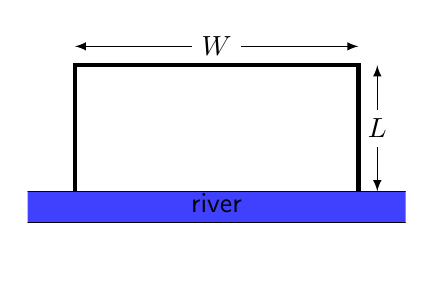
\begin{tikzpicture}[x=12mm,y=8mm,>=latex]
        \draw[thin,black,<->] (0,2.3) -- (3,2.3) node[midway,fill=white] {$W$};
        \draw[thin,black,<->] (3.2,0) -- (3.2,2) node[midway,fill=white] {$L$};
        \draw[ultra thick,black] (0,0) -- (0,2) -- (3,2) -- (3,0);
        \begin{scope}
          \clip (-0.5,0.5) rectangle (3.5,-1);
          \draw[thin,black,fill=blue!75] (-1,0) rectangle (4,-0.5);
          \node[above] at (1.5,-0.5) {\textsf{river}};
        \end{scope}
      \end{tikzpicture}
    \end{center}
  }
}


\frame{
  \frametitle{Word Problem \#4}

  Tickets are going to be sold for a concert.
  \begin{itemize}
  \item If the price of each  ticket is \$40, then $2,000$ tickets
    will be sold. 

  \item For every \$1 the price is decreased, $100$ more tickets will
    be sold.  
  \end{itemize}

  \begin{enumerate}
  \item[\colorbox{blue!50}{(a)}]\ 
    If the tickets are sold for $\$x$ each, how many will be sold?
    \vspace*{-0.5em}

    \begin{center}
      A $=2000-x$
      \quad 
      B $= 2000-100x$
      \quad 
      C $= 2000+100x$\\[0.5em]
      \ \quad\quad\quad
      D $= 6000-100x$
      \quad 
      E $=6000+100x$
      \pause
      \quad\quad\quad
      \fbox{D}
    \end{center}
    \vspace*{-0.5em}
    % \medskip

  \item[\colorbox{blue!50}{(b)}]\ 
    What is the total amount of money generated from selling tickets
    for $\$x$ each? 
    \vspace*{-0.5em}

    \begin{center}
      A $=6000x-100x^2$
      \quad 
      B $= 2000x$
      \\[0.5em]
      \ 
      \quad 
      C $= 2000-40x^2$
      \quad 
      D $=  6000-100x$
      \pause
      \quad
      \fbox{A}
    \end{center}
    \vspace*{-0.5em}
    % \medskip

  \item[\colorbox{blue!50}{(c)}]\ 
    What price should the tickets be to generate the most money from
    sales? 
    \vspace*{-0.5em}

    \begin{center}
      A $=\$20$
      \quad 
      B $= \$22$
      \quad 
      C $= \$24$
      \quad 
      D $= \$30$
      \quad 
      E $= \$40$
      \pause
      \quad
      \fbox{D}
    \end{center}
    % \bigskip
  \end{enumerate}

}



\frame{
  \frametitle{Word Problem \#5}
  
  A farmer is growing wheat.
  \begin{itemize}
  \item On July 1, she has $1,000$ bushels and this increases by $50$
    bushels per day. 

  \item The price of a bushel on July 1 is $\$10$ and is dropping at a rate of $20$ cents per day. 

  \item She will harvest and sell on the same day. 
  \end{itemize}
  How many days should she wait, assuming these trends continue?
  \begin{center}
    A $= 5$
    \quad 
    B $= 10$
    \quad 
    C $= 15$
    \quad 
    D $= 20$
    \quad 
    E $= \text{other}$
    \pause
    \quad
    \fbox{C}
  \end{center}
  \vspace*{2in}

}


\section{Review Problems}

\frame{
  \frametitle{Review Problems (page 1)}

  \begin{enumerate}
  \item Find the equation of the tangent line to $y=x^3-5x$ at $x=2$. 

    \begin{center}
      A\ $y=2x-6$
      \quad 
      B\ $y=16x-7$
      \quad 
      C\ $y= 7x+16$
      \quad 
      D\ $y = 7x-16$
    \end{center}

    \uncover<2->{%
      \begin{center}
        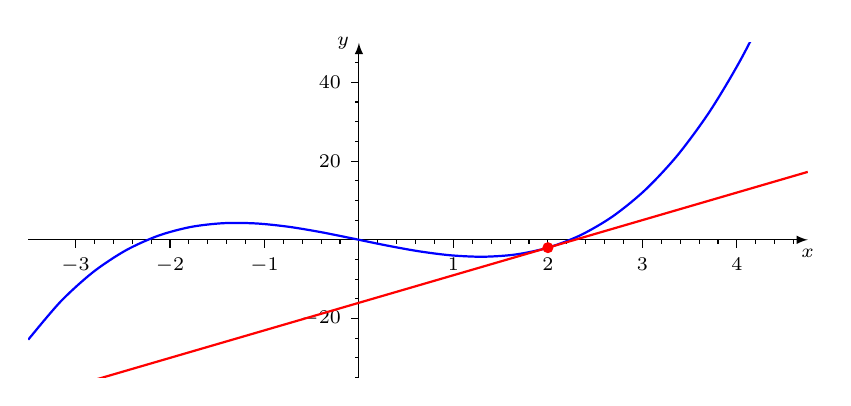
\begin{tikzpicture}[x=12mm,y=0.5mm,>=latex]
          \draw[thin,black,->] (-3.5,0) -- (4.75,0) node[below] {$\scriptstyle{}x$};
          \draw[thin,black,->] (0,-35) -- (0,50) node[left] {$\scriptstyle{}y$};
          % ticks:
          \foreach \x in {-3,-2,-1,1,2,3,4}
          {
            \draw[thin,black] (\x,0) -- (\x,-3pt) node[below] {$\scriptstyle\x$};
          }
          \foreach \x in {-3,-2.8,...,4.6}
          {
            \draw[thin,black] (\x,0) -- (\x,-1.5pt);
          }
          \foreach \y in {-20,20,40}
          {
            \draw[thin,black] (0,\y) -- (-3pt,\y) node[left] {$\scriptstyle\y$};
          }
          \foreach \y in {-35,-30,...,45}
          {
            \draw[thin,black] (0,\y) -- (-1.5pt,\y);
          }
          \begin{scope}
            \clip (-3.5,-35) rectangle (4.75,50);
            \draw[thick,blue,domain=-3.5:4.75,smooth] plot (\x,{(\x)^3-5*\x});
            \uncover<3->{%
              \draw[thick,red,domain=-3.5:4.75,smooth] plot (\x,{7*\x-16});
            }
            \fill[red] (2,-2) circle (2pt);
          \end{scope}
        \end{tikzpicture}
      \end{center}
    }
  \end{enumerate}
  \uncover<4->{\alert{Answer:}\ \answer{D}}

  \vspace*{2in}

}

\end{document}

\frame{
  \frametitle{Review Problems (page 2)}

  \begin{enumerate}
    \setcounter{enumi}{1}
  \item Where is $f(x)=3x^2+12x-4$ decreasing?
    \begin{center}
      A\ $x < -2$
      \quad 
      B\ $x > -2$
      \quad 
      C\ $x < 2$
      \quad 
      D\ $x > 2$
      \quad 
      E\ $x=2$
    \end{center}
  \end{enumerate}
  % \bigskip

  \uncover<2->{%
    \begin{center}
      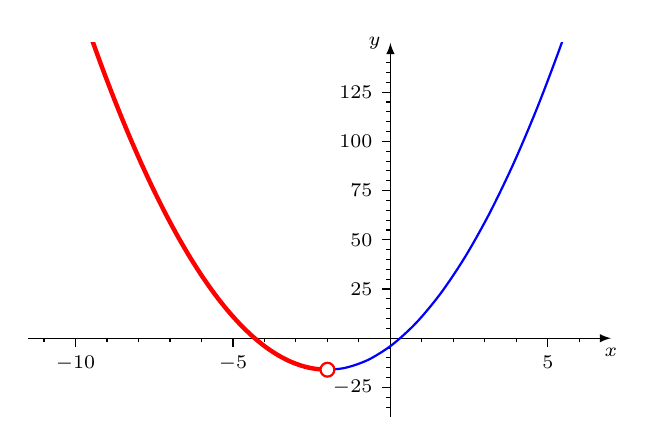
\begin{tikzpicture}[x=4mm,y=0.25mm,>=latex]
        \draw[thin,black,->] (-11.5,0) -- (7,0) node[below] {$\scriptstyle{}x$};
        \draw[thin,black,->] (0,-40) -- (0,150) node[left] {$\scriptstyle{}y$};
        % ticks:
        \foreach \x in {-10,-5,5}
        {
          \draw[thin,black] (\x,0) -- (\x,-3pt) node[below] {$\scriptstyle\x$};
        }
        \foreach \x in {-11,-10,...,6}
        {
          \draw[thin,black] (\x,0) -- (\x,-1.5pt);
        }
        \foreach \y in {-25,25,50,75,100,125}
        {
          \draw[thin,black] (0,\y) -- (-3pt,\y) node[left] {$\scriptstyle\y$};
        }
        \foreach \y in {-35,-30,...,140}
        {
          \draw[thin,black] (0,\y) -- (-1.5pt,\y);
        }
        \begin{scope}
          \clip (-11.5,-40) rectangle (7,150);
          \draw[thick,blue,domain=-11.5:7,smooth] plot (\x,{3*(\x)^2+12*\x-4});
          \uncover<3->{%
            \draw[ultra thick,red,domain=-11.5:-2,smooth] plot (\x,{3*(\x)^2+12*\x-4});
            \draw[thick,red,fill=white] (-2,-16) circle (2.5pt);
          }
        \end{scope}
      \end{tikzpicture}
    \end{center}
  }
  \uncover<4->{\alert{Answer:}\ \answer{A}}

  \vspace*{2in}


}

\frame{
  \frametitle{Review Problems (page 3)}

  \begin{enumerate}
    \setcounter{enumi}{2}
    \item Where is $f(x)=x^3 + 12 x^2 + 6x + 18$ concave up? 
      \begin{center}
        A\ $x< -4$
        \quad 
        B\ $x >-4$
        \quad 
        C\ $x > -2$
        \quad 
        D\ $x < -2$ 
      \end{center}
  \end{enumerate}

  \uncover<2->{%
  \begin{center}
    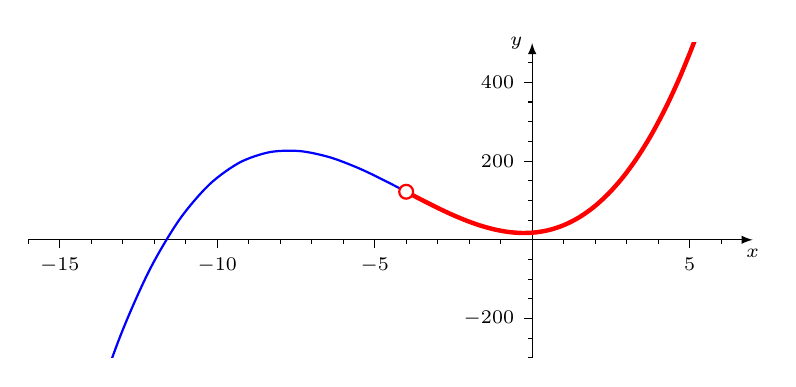
\begin{tikzpicture}[x=4mm,y=0.05mm,>=latex]
      \draw[thin,black,->] (-16,0) -- (7,0) node[below] {$\scriptstyle{}x$};
      \draw[thin,black,->] (0,-300) -- (0,500) node[left] {$\scriptstyle{}y$};
      % ticks:
      \foreach \x in {-15,-10,-5,5}
      {
        \draw[thin,black] (\x,0) -- (\x,-3pt) node[below] {$\scriptstyle\x$};
      }
      \foreach \x in {-16,-15,...,6}
      {
        \draw[thin,black] (\x,0) -- (\x,-1.5pt);
      }
      \foreach \y in {-200,200,400}
      {
        \draw[thin,black] (0,\y) -- (-3pt,\y) node[left] {$\scriptstyle\y$};
      }
      \foreach \y in {-300,-250,...,450}
      {
        \draw[thin,black] (0,\y) -- (-1.5pt,\y);
      }
      \begin{scope}
        \clip (-16,-300) rectangle (7,500);
        \draw[thick,blue,domain=-16:7,smooth] plot (\x,{(\x)^3+12*(\x)^2+6*\x+18});
        \uncover<3->{%
          \draw[ultra thick,red,domain=-4:7,smooth] plot (\x,{(\x)^3+12*(\x)^2+6*\x+18});
          \draw[thick,red,fill=white] (-4,122) circle (2.5pt);
        }
      \end{scope}
    \end{tikzpicture}
  \end{center}
  }
  \uncover<3->{\alert{Answer:}\ \answer{B}}


}









\end{document}
